\documentclass[a4paper,10pt]{article}
\usepackage[utf8]{inputenc}
\usepackage[czech]{babel}
\usepackage{graphicx}
\usepackage{tabularx}

\newcommand\floor[1]{\lfloor#1\rfloor}

\title{\bfseries Řešení problému vážené splnitelnosti booleovské formule pokročilou iterativní metodou}
\author{Bc. Marek Dostál, ČVUT}

\begin{document}

\maketitle
%\noindent\rule[0.5ex]{\linewidth}{0.1pt}

\section*{Boolean satisfiability problem}

Je dána booleovská formule $F$ proměnnných $X=(x_1, x_2, … , x_n)$ v konjunktivní normální
formě (tj. součin součtů). Dále jsou dány celočíselné kladné váhy $W=(w_1, w_2, … , w_n)$.
Najděte ohodnocení $Y=(y_1, y_2, … , y_n)$ proměnných $x_1, x_2, … , x_n$ tak, aby $F(Y)=1$
a součet vah proměnných, které jsou ohodnoceny jedničkou, byl maximální.

Je přípustné se omezit na formule, v nichž má každá klauzule právě 3 literály (problém 3 SAT).
Takto omezený problém je stejně těžký, ale možná se lépe programuje a lépe se posuzuje
obtížnost instance (viz Selmanova prezentace~\cite{edux-solman}).

\section*{Specifikace úlohy}

\begin{itemize}
\item Problém řešte některou z pokročilých lokálních heuristik (simulované ochlazování,
genetické algoritmy, tabu prohledávání).
\item Volby konkrétních parametrů heuristiky a jejích detailů (operace nad stavovým prostorem,
kritérium ukončení, atd.) proveďte sami, tyto volby pokud možno zdůvodněte a ověřte
experimentálním vyhodnocením.
\end{itemize}

\section*{Testovací data}

Data byla získána z DIMACS archivu \cite{edux-dimacs} a obohacena o náhodně vygenerované váhy v rozmezí od 0 do 100.
Skript pro generování je součástí odevzdaného projektu. Většina měření probíhala na datech s 50 proměnnými ($n$)
a 218 klauzulí, příp. 20/91.

\section*{Realizace řešení}

Pro řešení problému jsem si vybral heuristiku simulované ochlazování, kterou
jsem popsal detailně již v minulém čtvrtém úkolu.
Za připomínku stojí připomenout, že algoritmus má tři vstupní parametry:

\begin{itemize}
  \item počáteční teplota $t$
  \item faktor ochlazování $c$ (číslo z intervalu 0 až 1, kterým se teplota násobí)
  \item počet kroků před každým snížením teploty $i$
\end{itemize}

Na rozdíl od Knapsack problému musíme pozměnit cenovou funkci. Nestačí sečíst ceny nebo váhy položek vložených do batohu, ale je
potřeba lépe nechat projevit skutečnost, zda $F(Y)=1$. Protože nalezení takové
konfigurace není triviální úkol, musíme začít prohledávat i takové stavy, které tuto
podmínku nesplňují. V každém případě cenová funkce v~mém případě je následující:

$$h(H)= k\frac{C_X}{C_{total}} + (1-k)\frac{W_X}{W_{total}}$$

kde $\frac{C_X}{C_{total}}$ je poměr mezi splněnými a všemi klauzulemi (dosažená splnitelnost). Druhý zlomek je
poměrem využité a dostupné váhy (využítí váhy). Konstanta $k$ přiřazuje důležitost oběma poměrům.

Cenová funkce je omezujícím faktorem, proč je moje řešení vhodné pouze pro 3-SAT. Funkce by musela
přikládat různým klauzulím různá ohodnocení. Splnit větší klauzule je totiž jednodušší než ty menší.

Výsledky měření byly zaznamenány na počítači s OS Ubuntu 14.04 a procesorem Intel Core M (Broadwell) 5Y10(0.8/2GHz).
Program, implementovaný v~jazyce Python, zkoušel vždy 50 různých instancí pro vybrané $n$.

\subsection*{Best state}

Pro výrazné zlepšení účinnosti byla implementovaná velmi drobná avšak účinná změna.
Při prochazení stavů si ukladám ten doposud nejlepší a tím mám zajištěnou vlastnost, že po dosažení globálního maxima
můžu bez váhání hledat v jeho okolí i za cenu, že z něj \uv{vyskočím}. Algoritmus tak na konci vrátí nejlepší dosažený
výsledek v rámci celého svého běhu. Pro ověření jsem provedl drobné měření.

Na 50 instancích s $n=20$, $t=1000$, $c=0.85$, $i=1000$, $k=0.85$ a koncové teplotě 1 jsem dosáhl těchto hodnot:

\renewcommand{\arraystretch}{1.15}
\begin{table}[htb]
 \centering
\begin{tabular}{ c || c | c | c | c | c | c}
  & \textbf{s ukládáním nejlepší stavu} & \textbf{bez ukládání} \\
  \hline
využítí váhy & 0.62963 \% & 0.49655 \% \\
dosažená splnitelnost & 0.98791 \% & 0.87759  \%\\
průměrný čas & 2545.08797 ms & 2640.91332 ms\\
\end{tabular}
\end{table}

Pokud by nás trápilo, že v mnoha případech nedosáhneme 100\% splitelnosti, tzn. $F(Y)=1$,
mohli bychom buď upravit vstupní konstantu $k$ na vyšší hodnotu či přidat podmínku,
že nejlepší dosažený stav může být pouze ten, který splňuje 100\% splitelnost nebo
si v ní minimálně nepohoršuje.

Z několika předchozích pokusů jsem usoudil, že pro následující měření bude vhodné ponechat výše uvedené parametry.

\subsection*{Závislost dosažených výsledků}

V prvních třech grafech si můžeme všimnout podobných vlastností. Parametry nás sice
pomalu přibližují optimálnímu řešení, ale bohužel velmi pomalu. Navíc pokud vezmeme v potaz,
že vyšší hodnoty vstupních parametrů prodlužují běh algoritmu, jak si později ukážeme,
je potřeba jejich využití zvážit. Všimněme si však o něco rychlejšího růstu ve využití celkové váhy.

\subsubsection*{na velikosti vnitřní smyčky}
\begin{center}
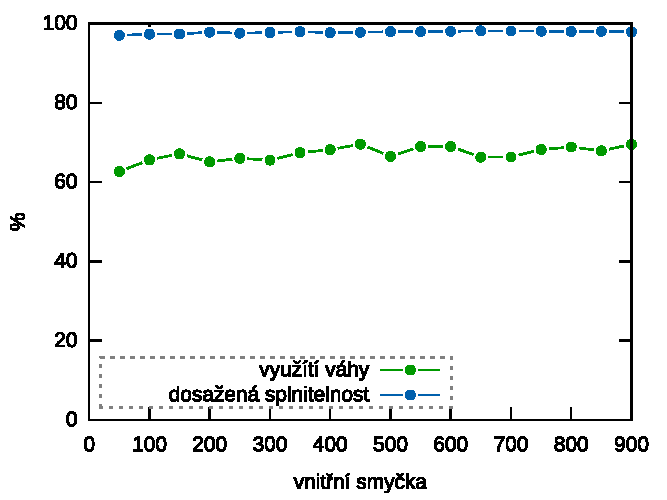
\includegraphics[width=0.8\textwidth]{inner_loop.pdf}
\end{center}
\subsubsection*{na chlazení}
\begin{center}
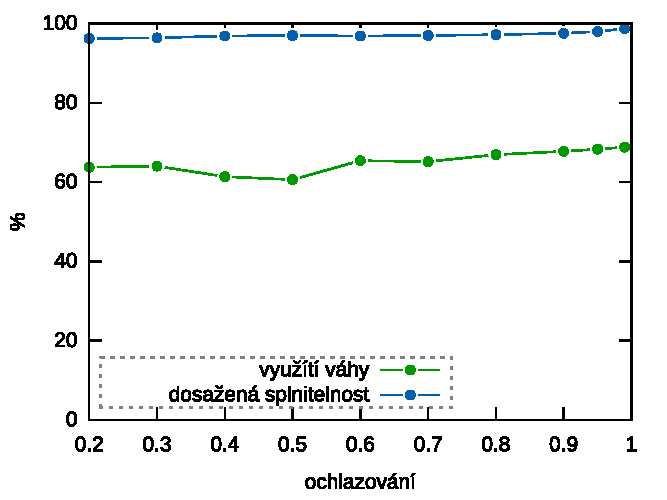
\includegraphics[width=0.8\textwidth]{ochlazovani.pdf}
\end{center}
\subsubsection*{na teplotě}
\begin{center}
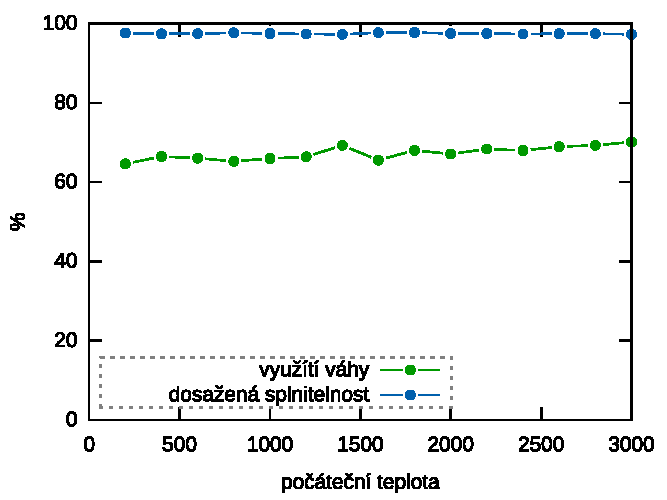
\includegraphics[width=0.8\textwidth]{teplota.pdf}
\end{center}
\subsubsection*{na konstantě $k$}
Zde vidíme první zajímavé chování. Avšak ne překvapivé. Konstanta nám vlastně říká, jakému poměru se máme více věnovat.
Na konci proto vidíme rozevřené nůžky, kde se výsledek snaží maximálně dosáhnout podmínky $F(Y)=1$, ale za cenu toho,
že přestává cílit na proměnné s vyšší váhou.
\begin{center}
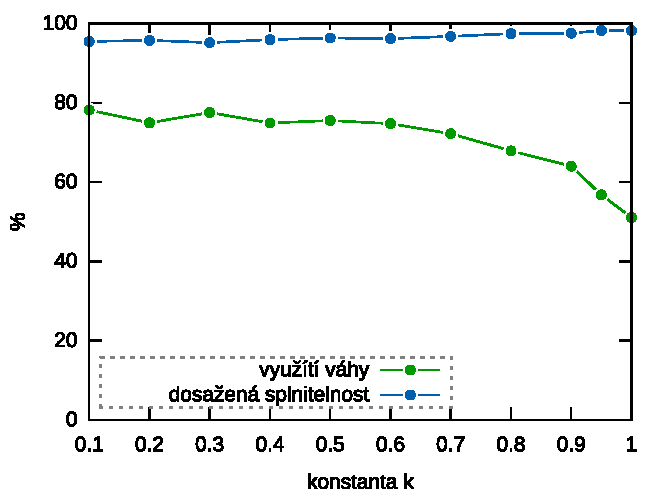
\includegraphics[width=0.8\textwidth]{k.pdf}
\end{center}

\subsection*{Závislost výpočetního času}

V této části se nám potvrdili meření ze čtvrtého úkolu. Teplota a vnitřní smyčka mohou úlohu
výrazně prodlužovat. Příliš nízké ochlazování jej může prodloužit dokonce až exponenciálně.
Graf popisující závislost u konstanty $k$ ukazuje naprostou nezávislost na aktuální hodnotě.

\subsubsection*{na velikosti vnitřní smyčky}
\begin{center}
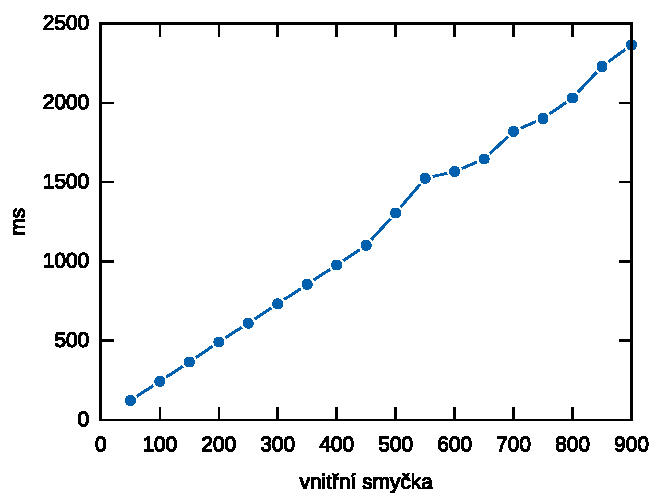
\includegraphics[width=0.8\textwidth]{inner_loop_time.pdf}
\end{center}
\subsubsection*{na chlazení}
\begin{center}
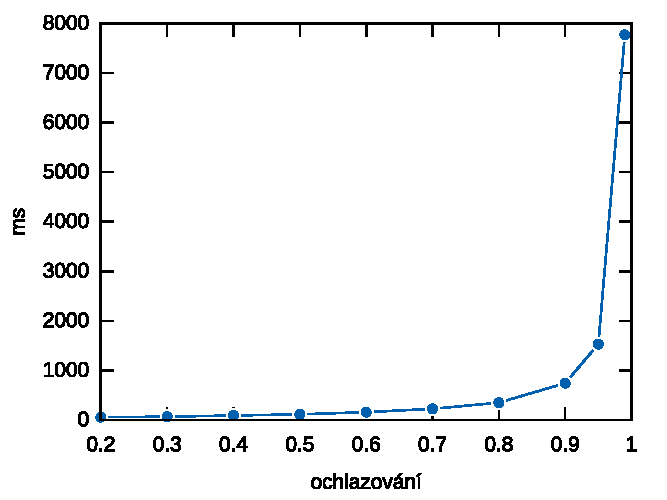
\includegraphics[width=0.8\textwidth]{ochlazovani_time.pdf}
\end{center}
\subsubsection*{na teplotě}
\begin{center}
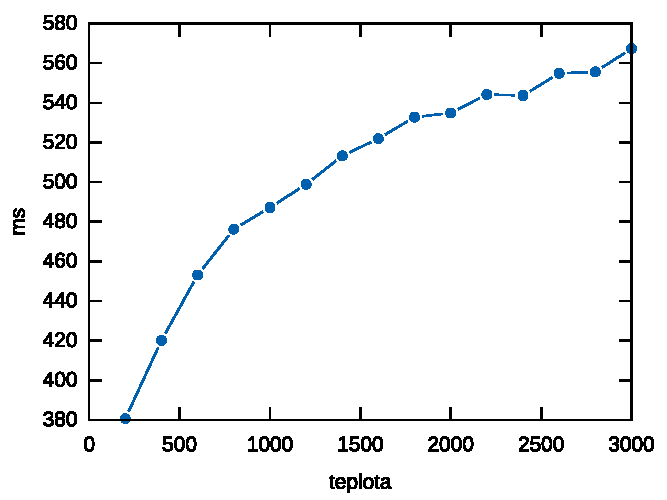
\includegraphics[width=0.8\textwidth]{teplota_time.pdf}
\end{center}
\subsubsection*{na konstantě $k$}
\begin{center}
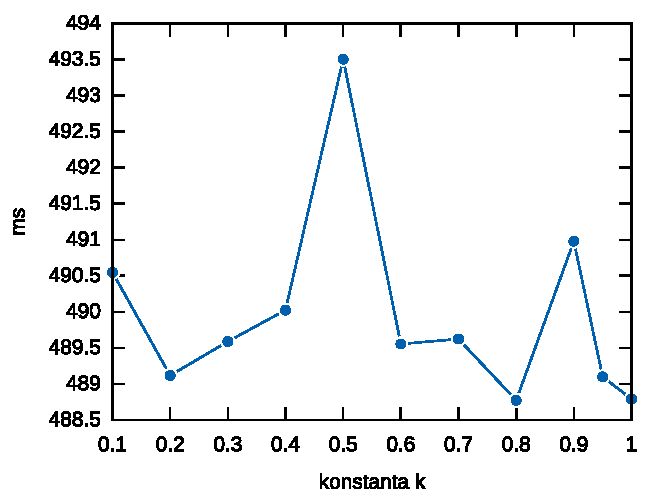
\includegraphics[width=0.8\textwidth]{k_time.pdf}
\end{center}

\section*{Závěr}

Řešení určitě pomohlo ukládání si nejlepšího dosaženého stavu. Avšak za celou dobu měření se nepovedlo
nastavit vstupní parametry tak, abych dosáhl lepších výsledků u větších instancí.
V mnoha případech se mi nedařilo nalézt takové řešení, které by splňovalo podmínku $F(Y)=1$, protože se
algoritmus často \uv{zasekl} v lokálním maximu. Možná by pomohlo změnit cenovou funkci~$h$.
To se netýkalo instancí s $n=20$, kde byla úspěšnost nalezení řešení skoro 100\%.
Jak blízko optimálnímu řešení jsem byl s využitím váhy není bohužel možné zjistit, protože k datům chyběla správná řešení.

\renewcommand{\refname}{Použité zdroje}
\begin{thebibliography}{9}


\bibitem{edux-sat}
  Problém. Řešení problému vážené splnitelnosti booleovské formule pokročilou iterativní metodou.
  EDUX: MI-PAA Problémy a algoritmy [online]. 2011/09/18
  \mbox{[cit. 2017-02-02]}.
  Dostupné z: https://edux.fit.cvut.cz/courses/MI-PAA/homeworks/05/start
  
\bibitem{edux-solman}
  http://www.cs.cornell.edu/home/selman/papers-ftp/ai-phys1.ppt

\bibitem{edux-dimacs}
  http://www.cs.ubc.ca/~hoos/SATLIB/benchm.html
  
\end{thebibliography}

\end{document}
